\documentclass{standalone}
\usepackage{tikz}
\begin{document}%
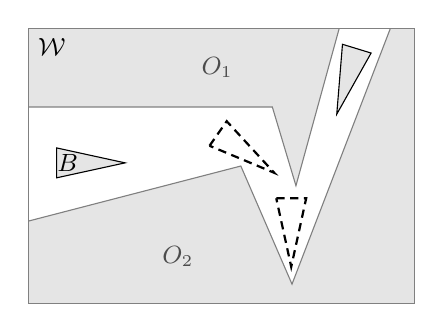
\begin{tikzpicture}[font=\small]

% obstacles
\fill[black!10] (0.0,3.5) -- (3.95,3.5) -- (3.40,1.50)
   -- (3.1,2.5) -- (0.0,2.50) -- cycle;
\fill[black!10] (0.0,0.0) -- (0.0,1.05) -- (2.7,1.75)
   -- (3.35,0.25) -- (4.60,3.5) -- (4.9,3.5) -- (4.9,0.0) -- cycle;
% obstacle borders
\draw[black!50] (3.95,3.5) -- (3.40,1.50) -- (3.1,2.5) -- (0.0,2.50);
\draw[black!50] (0.0,1.05) -- (2.7,1.75) -- (3.35,0.25) -- (4.60,3.5);
% body left
\begin{scope}[shift={(0.1,-0.3)},rotate=0]
   \filldraw[fill=black!10,draw=black] (0.26,1.90) -- (0.26,2.28) -- (1.13,2.09) -- cycle;
\end{scope}
% body middle left
\begin{scope}[shift={(1.0,0.6)},rotate=-35]
   \draw[draw=black,densely dashed,thick] (0.26,1.90) -- (0.26,2.28) -- (1.13,2.09) -- cycle;
\end{scope}
% body middle right
\begin{scope}[shift={(1.25,1.6)},rotate=-90]
   \draw[draw=black,densely dashed,thick] (0.26,1.90) -- (0.26,2.28) -- (1.13,2.09) -- cycle;
\end{scope}
% body right
\begin{scope}[shift={(2.25,4.1)},rotate=-107]
   \filldraw[fill=black!10,draw=black] (0.26,1.90) -- (0.26,2.28) -- (1.13,2.09) -- cycle;
\end{scope}

% obstacle labels
\node[text=black!70] at (2.4,3.0) {$O_1$};
\node[text=black!70] at (1.9,0.6) {$O_2$};

% body label
\node[text=black] (blab) at (0.5,1.79) {$B$};

% W label
\node[text=black,anchor=north west] at (0.0,3.5) {$\mathcal{W}$};

% W-space border
\draw[black!50] (0,0) rectangle (4.9,3.5);

\end{tikzpicture}%
\end{document}
